% Author: Seongjin Lee
% Hanyang University, Seoul, Korea
% esos.hanyang.ac.kr
% 2016-09-20
% note: some slides are adopted from  \url{www.cs.stevens.edu/~jschauma/631A/}
% https://github.com/resourceful/lecture_sysprog/

\documentclass[newPxFont,sthlmFooter,nooffset]{beamer}
\usepackage{kotex}
%\usetheme{sthlm}
\usepackage{../beamer_template/beamerthemesthlm}
\hypersetup{pdfauthor={Seongjin Lee (insight@gnu.ac.kr)},
            pdfsubject={Lecture Note: System Programming},
            pdfkeywords={Lecture Note, System Programming, class, (under)graduate},
            pdfmoddate={D: \pdfdate},
            pdfcreator={Seongjin Lee}}

%\setbeamertemplate{footline}[text line]{%
%    \parbox{\linewidth}{\vspace*{-8pt} \insertsectionhead  \hfill\insertshortauthor\hfill\insertpagenumber}}
%\setbeamertemplate{navigation symbols}{}




\title{System Programming}
\subtitle{Topic 10: Interprocess Commnunication}
\author[SJL]{Seongjin Lee}
\institute{\href{mailto:insight@gnu.ac.kr}{insight@gnu.ac.kr}\\\url{http://open.gnu.ac.kr}\\Systems Research Lab.\\Gyeongsang National University}
\date{\today}

\begin{document}



\frame[plain]{\titlepage}

\frame[t]{\frametitle{Table of contents}\tableofcontents}


%---------------------------------------------------------



\begin{frame}[t]
  \frametitle{Introduction}



This chapter covers other techniques for processes to communicate with one another: interprocess communication (IPC)
\begin{itemize}
\item pipes
\item FIFOs
\item Message Queues
\item Shared Memory
\item Semaphores
\end{itemize}
\end{frame}

\section{Pipes}

\begin{frame}[t, fragile]
  \frametitle{Pipes}
Pipes are the oldest form of \textsc{Unix} system IPC

Pipes have two limitations
\begin{enumerate}
\item They have been half duplex (most commonly used), now provide full-duplex pipes (but never assume it is full-duplex)
\item Pipes can be used only between processes that have a common ancestor
\end{enumerate}

\end{frame}


\begin{frame}[t, fragile]
  \frametitle{Pipes}
\begin{codedef}
#include <unistd.h>
int pipe(int fd[2]);
// Returns: 0 if OK, −1 on error
\end{codedef}
Two file descriptors are returned through the fd argument:
\begin{itemize}
\item \texttt{fd[0]} is open for reading,
\item \texttt{fd[1]} is open for writing.
\item The output of \texttt{fd[1]} is the input for \texttt{fd[0]}.
\end{itemize}

\end{frame}



\begin{frame}[t]
  \frametitle{Pipes}
  \begin{figure}[h]
    \centering
    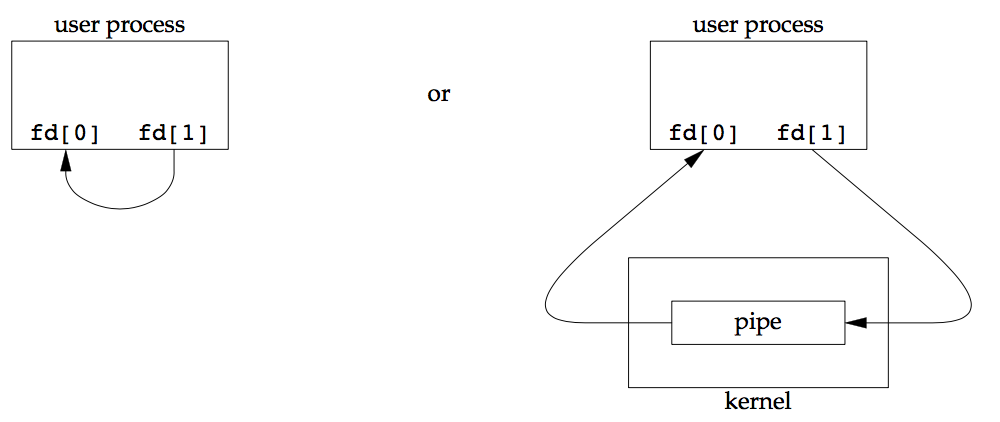
\includegraphics[width=0.8\textwidth]{./figures/fig15_2-twoways.png}
    \caption{Two ways to veiw a half-duplex pipe}
  \end{figure}


\end{frame}



\begin{frame}[t]
  \frametitle{Pipes}
Normally, the process that calls pipe then calls fork, creating an IPC channel from the parent to the child, or vice versa.
  \begin{figure}[h]
    \centering
   \only<1>{ 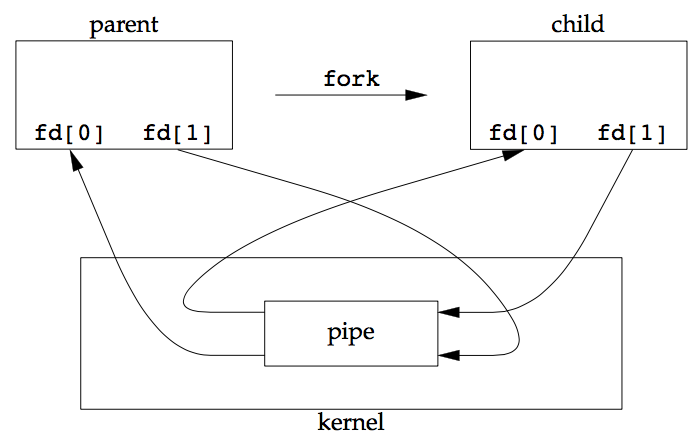
\includegraphics[width=0.8\textwidth]{./figures/fig15_3-halfduplex.png}
    \caption{Half-duplex pipe after a fork}}
  \only<2>{ 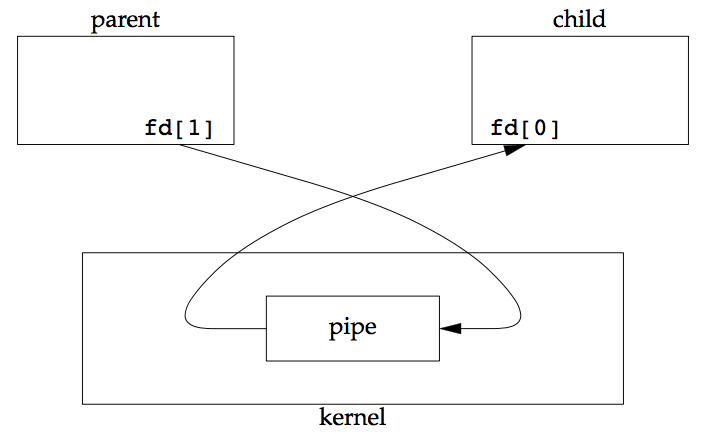
\includegraphics[width=0.8\textwidth]{./figures/fig15_4-pipe.png}
    \caption{Pipe from parent to child}}

  \end{figure}

\end{frame}



\begin{frame}[t]
  \frametitle{Pipes}
When one end of a pipe is closed, two rules apply
\begin{enumerate}
\item If we read from a pipe whose write end has been closed, read returns 0 to indicate an end of file after all the data has been read.
\item If we write to a pipe whose read end has been closed, the signal SIGPIPE is generated.
\end{enumerate}

When we’re writing to a pipe (or FIFO), the constant \texttt{PIPE\_BUF} specifies the kernel’s pipe buffer size.
\end{frame}



\begin{frame}[t, fragile, allowframebreaks]
  \frametitle{Pipes Example: \texttt{codes/pipe1.c}}
In this example, we call \texttt{read} and \texttt{write} directly on the pipe descriptors.

\lstinputlisting[lineskip=0pt]{codes/pipe1.c}
\end{frame}



\begin{frame}[t, fragile, allowframebreaks]
  \frametitle{Pipes Example: \texttt{codes/pipe2.c}}

  \begin{itemize}
  \item Before calling fork, we create a pipe.
  \item After the fork, the parent closes its read end, and the child
    closes its write end.
  \item The child then calls dup2 to have its
    standard input be the read end of the pipe.
  \item When the pager program
    is executed, its standard input will be the read end of the pipe.
  \end{itemize}


\lstinputlisting[lineskip=0pt]{codes/pipe2.c}

\begin{block}{Defensive programming measure}
Whenever we call dup2 and close to duplicate one descriptor onto another, we’ll always compare the descriptors first.
\end{block}
\end{frame}

\subsection{\texttt{popen} and \texttt{pclose} Functions}

\begin{frame}[t, fragile]
  \frametitle{\texttt{popen} and \texttt{pclose} Functions}
Standard I/O library to create a pipe to another process to either read or write
\begin{codedef}
#include <stdio.h>
FILE *popen(const char *cmdstring, const char *type);

// Returns: file pointer if OK, NULL on error

int pclose(FILE *fp);
// Returns: termination status of cmdstring, or −1 on error
\end{codedef}

The function \texttt{\texttt{popen}} does a \texttt{fork} and \texttt{exec} to execute the \textit{cmdstring} and returns a standard I/O file pointer.
\end{frame}



\begin{frame}[t]
  \frametitle{\texttt{popen} and \texttt{pclose} Functions}

If \textit{type} is ``\texttt{r}'', the file pointer is connected to the standard output of \textit{cmdstring}
  \begin{figure}[h]
    \centering
    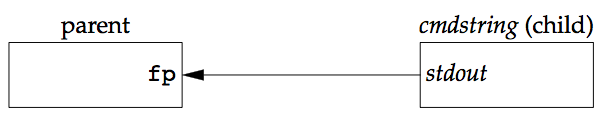
\includegraphics[width=0.5\textwidth]{./figures/fig15_9-result-r.png}
    \caption{Result of \texttt{fp = popen}(\texttt{cmdstring}, \texttt{``r''})}
  \end{figure}

If \texttt{type} is ``\texttt{w}'', the file pointer is connected to the standard input of \textit{cmdstring}
  \begin{figure}[h]
    \centering
    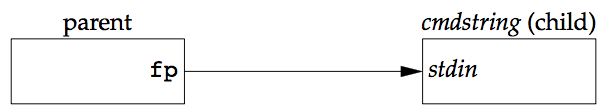
\includegraphics[width=0.5\textwidth]{./figures/fig15_10-result-w.png}

  \end{figure}

\end{frame}



\begin{frame}[t]
  \frametitle{\texttt{popen} and \texttt{pclose} Functions}
The \texttt{pclose} function closes the standard I/O stream, waits for the command to terminate, and returns the termination status of the shell.
\end{frame}



\begin{frame}[t, fragile, allowframebreaks]
  \frametitle{\texttt{popen} and \texttt{pclose} Example}
redo of the program using \texttt{popen}: \texttt{codes/popen2.c}

The shell command \texttt{\$\{PAGER:-more\}} says to use the value of the shell variable
\texttt{PAGER} if it is defined and non-null; otherwise, use the string more.

\lstinputlisting[lineskip=0pt]{codes/popen2.c}
\end{frame}



\begin{frame}[t, fragile]
  \frametitle{\texttt{popen} and \texttt{pclose} Example}
\texttt{codes/myuclc.c} : a filter program that changes upper cases to lower cases.

\lstinputlisting[lineskip=-2pt]{codes/myuclc.c}
\end{frame}



\begin{frame}[t, fragile, allowframebreaks]
  \frametitle{\texttt{popen} and \texttt{pclose} Example}
\texttt{codes/popen1.c}

\lstinputlisting[lineskip=0pt]{codes/popen1.c}
\end{frame}



\section{Coprocesses}

\begin{frame}[t]
  \frametitle{Coprocesses}
A \textsc{Unix} system filter is a program that reads from standard input and writes to standard output.

Filters are normally connected linearly in shell pipelines.

A filter becomes a \textit{coprocess} when the same program generates the filter's input and reads the filter output

  \begin{figure}[h]
    \centering
    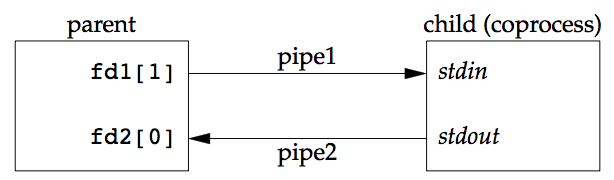
\includegraphics[width=0.5\textwidth]{./figures/fig15_16-driving.png}
    \caption{Driving a coprocess by writing its standard input and reading its standard output}
  \end{figure}


\end{frame}



\begin{frame}[t, fragile, allowframebreaks]
  \frametitle{Coprocess Example}
A simple coprocess that reads two numbers from its standard input, computes their sum, and writes the sum to its standard output.

\texttt{codes/add2.c; make add2}

\lstinputlisting[lineskip=-3pt]{codes/add2.c}

\bigskip

Here, we create two pipes, with the parent and the child closing the ends they don’t need.

\newpage
\texttt{codes/pipe4.c; make pipe4}
\lstinputlisting[lineskip=-3pt]{codes/pipe4.c}

\newpage
If we \texttt{kill} the \texttt{add2} coprocess while the program is waiting for our input and then enter two numbers, the signal handler is invoked when the program writes to the pipe that has no reader.

From another terminal type the following
\begin{codedefnb}
$ ps | grep add2
40467  ttys000  0:00.00 add2
$ kill 40467
\end{codedefnb}

then input two numbers to pipe4

\end{frame}

\section{FIFOs}

\begin{frame}[t]
  \frametitle{FIFOs}
FIFOs are sometimes called named pipes.
\begin{itemize}
\item FIFOs are sometimes called named pipes.
\item Unnamed pipes can be used only between related processes when a common ancestor has created the pipe.
\item With FIFOs, unrelated processes can exchange data.
\end{itemize}


\end{frame}



\begin{frame}[t, fragile]
  \frametitle{FIFOs}
Creating a FIFO is similar to creating a file. Indeed, the pathname for a FIFO exists in the file system
\begin{codedef}
 #include <sys/stat.h>
int mkfifo(const char *path, mode_t mode);
int mkfifoat(int fd, const char *path, mode_t mode);
// Both return: 0 if OK, −1 on error
\end{codedef}

\end{frame}



\begin{frame}[t]
  \frametitle{FIFOs}
\begin{itemize}
\item \textit{mode} argument is the same as for the open function (Section 3.3)
\item The rules for the user and group ownership of the new FIFO are the same as we described in Section 4.6
\item \texttt{mkfifoat} creates a FIFO in a location relative to the directory represented by the \texttt{fd} file descriptor argument.
{\footnotesize
  \begin{itemize}
  \item \textit{path} == absolute pathname: \texttt{mkfifoat} function behaves like the \texttt{mkfifo} function.
  \item \textit{path} == relative pathname $\&\&$ \texttt{fd} == valid directory: the pathname is evaluated relative to this directory.
  \item \textit{path} == relative pathname $\&\&$ \texttt{fd} == \texttt{AT\_FDCWD}: starts incurrent working directory, and mkfifoat behaves like mkfifo.
  \end{itemize}
}
\end{itemize}

Once we have used \texttt{mkfifo} or \texttt{mkfifoat} to create a FIFO, we open it using \texttt{open}. Indeed, the normal file I/O functions (e.g., close, \texttt{read}, \texttt{write}, \texttt{unlink}) all work with FIFOs.
\end{frame}


\begin{frame}[t]
  \frametitle{FIFOs}
When we open a FIFO, the nonblocking flag (\texttt{O\_NONBLOCK}) affects what happens.
\begin{itemize}
\item without \texttt{O\_NONBLOCK}:
  \begin{itemize}
  \item \texttt{open} for read-only blocks until some other process
    opens the FIFO for writing
  \item \texttt{open} for write-only blocks until some other process opens the FIFO for reading.
  \end{itemize}
\item with \texttt{O\_NONBLOCK}:
  \begin{itemize}
  \item  \texttt{open} for read-only returns immediately.
  \item \texttt{open} for write-only returns -1 with \texttt{errno} set to \texttt{ENXIO} if no process has the FIFO open for reading.
  \end{itemize}
\end{itemize}
\end{frame}



\begin{frame}[t]
  \frametitle{FIFO Use Cases}
There are two uses for FIFO
\begin{enumerate}
\item FIFOs are used by shell commands to pass data from one shell pipeline to another \textit{without creating intermediate temporary files}.
\item FIFOs are used as rendezvous points in client–server applications \texttt{to pass data between the clients and the servers}.
\end{enumerate}

\end{frame}



\begin{frame}[t]
  \frametitle{Example - Using FIFOs to Duplicate Output Streams}

FIFOs can be used to duplicate an output stream in a series of shell commands.

A FIFO has a name, so it can be used for nonlinear connections.
  \begin{figure}[h]
    \centering
    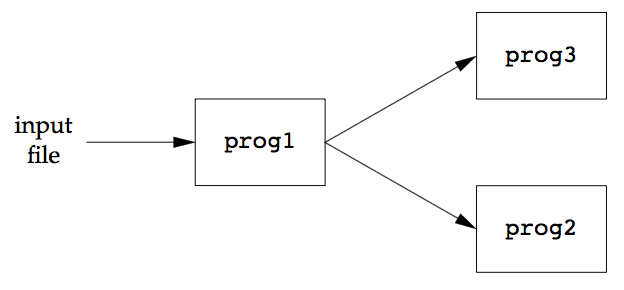
\includegraphics[width=0.5\textwidth]{figures/fig15_20-procedure.png}
    \caption{Procedure that processes a filtered input stream twice}
  \end{figure}


\end{frame}



\begin{frame}[t,fragile]
  \frametitle{Example - Using FIFOs to Duplicate Output Streams}
\begin{codedefnb}
mkfifo fifo1
prog3 < fifo1 &
prog1 < infile | tee fifo1 | prog2
\end{codedefnb}
  \begin{figure}[h]
    \centering
    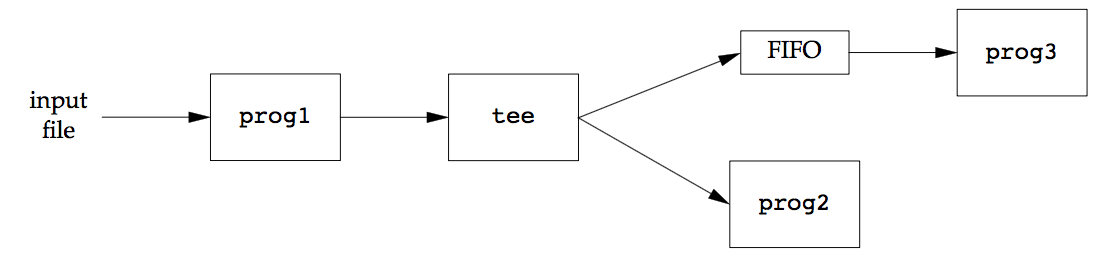
\includegraphics[width=1\textwidth]{figures/fig15_21-using.png}
    \caption{Using a FIFO and \texttt{tee} to send a stream to two different processes}
  \end{figure}

\end{frame}



\begin{frame}[t]
  \frametitle{Example - Client Server Communication Using FIFO}
  \begin{figure}[h]
    \centering
    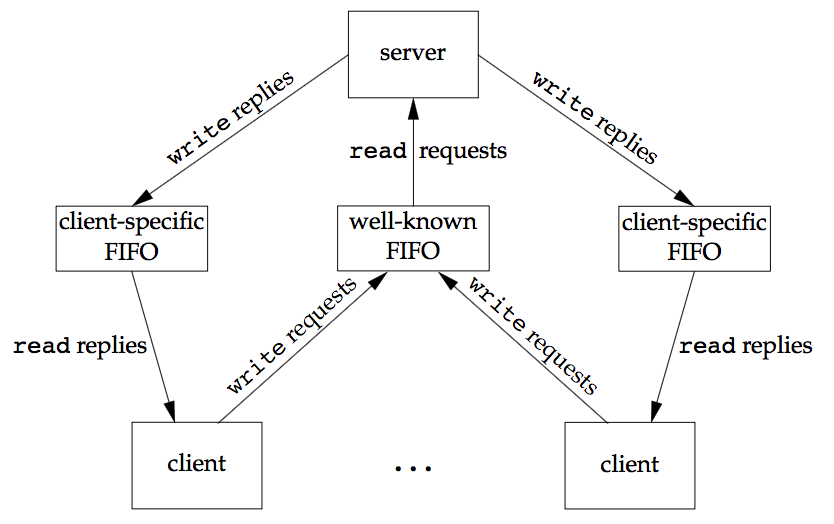
\includegraphics[width=1\textwidth]{figures/fig15_23-client.png}
    \caption{Client-server communication using FIFOs}
  \end{figure}

\end{frame}


\begin{frame}[t, fragile, allowframebreaks]
  \frametitle{Example - Client Server Communication Using FIFO}
\bigskip
\texttt{codes/create\_fifo.c}

\texttt{make create\_fifo} to create a FIFO for server and client

\lstinputlisting[lineskip=0pt]{codes/create_fifo.c}

\newpage
\bigskip
\texttt{codes/server.c}
\lstinputlisting[lineskip=-3pt]{codes/server.c}

\newpage
\bigskip
\texttt{codes/client.c}
\lstinputlisting[lineskip=-3pt]{codes/client.c}
\end{frame}

\section{XSI IPC}
\subsection{General Background}
\begin{frame}[t]
  \frametitle{XSI IPC}
There are three types of IPC that we call XSI IPC
\begin{enumerate}
\item message queues
\item semaphores
\item shared memory
\end{enumerate}
\end{frame}


\begin{frame}[t]
  \frametitle{Identifiers and Keys}
Each IPC \textit{structure} in the kernel is referred to by a non-negative integer \textit{identifier}
\begin{itemize}
\item to send a message to or fetch a message from a message queue, for example, all we need to know is the identifier for the queue
\item when a given IPC structure is created and then removed
  \begin{itemize}
  \item identifier associated with that structure conitunally increases
  \end{itemize}
\item identifier is an internal name for an IPC object
\end{itemize}
\end{frame}

\begin{frame}[t, fragile]
  \frametitle{Identifiers and Keys}
Whenever an IPC structure is being created, a key must be specified

\begin{codedef}
#include <sys/ipc.h>
key_t ftok(const char *path, int id);
// Returns: key if OK, (key_t)−1 on error
\end{codedef}

\begin{itemize}
\item \textit{path} must refer to an existing file
\item only the lower 8 bits of \textit{id} are used when generating the key
\item key created by \texttt{ftok} is foremd by taking parts of \texttt{st\_dev} and \texttt{st\_ino} fields in the \texttt{stat} structure
\end{itemize}

\end{frame}


\begin{frame}[t, fragile]
  \frametitle{Identifiers and Keys}
The three \texttt{get} functions (\texttt{msgget}, \texttt{semget}, and \texttt{shmget}) all have two similar arguments: a \textit{key} and an integer \textit{flag}


\bigskip
If we want to create a new unique IPC structure, we must specify a \textit{flag} with both the \texttt{IPC\_CREAT} and \texttt{IPC\_EXCL} bits set
\end{frame}

\begin{frame}[t, fragile]
  \frametitle{Permission Structure}
XSI IPC associates an \texttt{ipc\_perm} structure with each IPC structure

All the fields are initialized when the IPC structure is created

\texttt{\{msg | sem | shm\}ctl} can modify the \texttt{uid}, \texttt{gid}, and \texttt{mode} fields



\begin{columns}
  \begin{column}{0.7\textwidth}
\begin{codedefnb}
struct ipc_perm {
     uid_t  uid;  /* owner’s effective user ID */
     gid_t  gid;  /* owner’s effective group ID */
     uid_t  cuid; /* creator’s effective user ID */
     gid_t  cgid; /* creator’s effective group ID */
     mode_t mode; /* access modes */
     .
     .
     .
};
\end{codedefnb}
  \end{column}
  \begin{column}{0.3\textwidth}
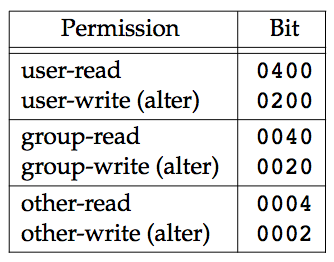
\includegraphics[width=\linewidth]{figures/fig15_24-xsi.png}
  \end{column}
\end{columns}
\end{frame}


\begin{frame}[t]
  \frametitle{IPC vs File}
  \begin{table}[h]
    \centering
    \begin{tabular}{c c c }
      File & $\longleftrightarrow$ & IPC \\ \hline
      File name & $\longleftrightarrow$ & Key \\
      file & $\longleftrightarrow$ & Object \\
      fd   & $\longleftrightarrow$ & Identifier
    \end{tabular}
  \end{table}

Difference between object identifiers and \texttt{fd}s
  \begin{itemize}
  \item IPC identifiers are kernel-persistent; \texttt{fd}s are process persistent
  \item IPC identifiers are globally visible; \texttt{fd}s are restricted to related processes
  \end{itemize}

\end{frame}


\begin{frame}[t]
  \frametitle{Advantages and Disadvantages}
Fundamental problem with XSI IPC:
  \begin{enumerate}
  \item IPC structures are systemwide and do not have a reference count
{\footnotesize
    \begin{itemize}
    \item After creating a message queue, place some messages on the queue, and the terminate, the message queue and its contents ar not deleted
    \item They remain until specifically read or deleted by \texttt{msgrcv} or \texttt{msgctl}, by executing the \texttt{ipcrm(1)} command, or by system being rebooted
    \end{itemize}
}
\item IPC structures are not kwown by names in the file system
{\footnotesize
  \begin{itemize}
  \item new system calls required (\texttt{msgget}, \texttt{semop}, \texttt{shmat}, and so on)
  \item can't see the IPC objects with \texttt{ls} command or remove them with \texttt{rm}; instead two new commands---\texttt{ipcs(1)} and \texttt{ipcrm(1)}---were added
  \end{itemize}
}
  \end{enumerate}

\end{frame}



\begin{frame}[t]
  \frametitle{Advantages and Disadvantages}
  \begin{figure}[h]
    \centering
    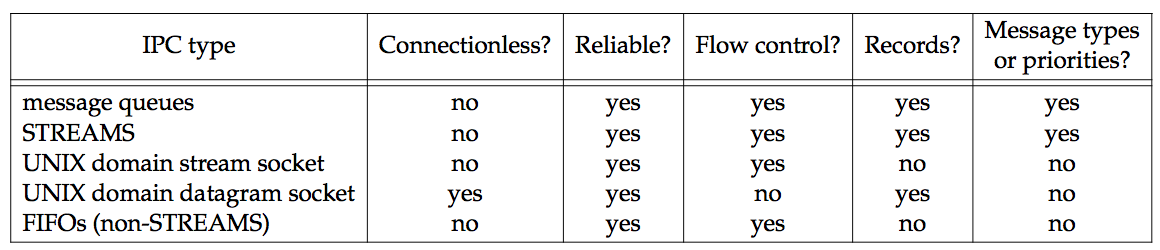
\includegraphics[width=\linewidth]{figures/fig15_25-comparison.png}
    \caption{Comparison of features of various forms of IPC}
  \end{figure}

By ``connectionless,'' we mean the ability to send a message without having to call some form of an open function first

``Flow control'' means that the sender is put to sleep if there is a shortage of system resources (buffers) or if the receiver can’t accept any more messages.
\end{frame}


\subsection{XSI Message Queues}
\begin{frame}[t]
  \frametitle{Message Queues}
A message queue is a linked list of messages stored within the kernel and identified by a message queue identifier.
\begin{itemize}
\item A new queue is created or an existing queue opened by \texttt{msgget}.
\item New messages are added to the end of a queue by \texttt{msgsnd}.
\item Messages are fetched from a queue by \texttt{msgrcv}.
\item We don’t have to fetch the messages in a first-in, first-out order. Instead, we can fetch messages based on their type field.
\end{itemize}
\end{frame}



\begin{frame}[t, fragile]
  \frametitle{Message Qeues Datastructure}
\begin{codedefnb}
struct msqid_ds {
  struct ipc_perm  msg_perm;   /* see Section 15.6.2 */
  msgqnum_t        msg_qnum;   /* # of messages on queue */
  msglen_t         msg_qbytes; /* max # of bytes on queue */
  pid_t            msg_lspid;  /* pid of last msgsnd() */
  pid_t            msg_lrpid;  /* pid of last msgrcv() */
  time_t           msg_stime;  /* last-msgsnd() time */
  time_t           msg_rtime;  /* last-msgrcv() time */
  time_t           msg_ctime;  /* last-change time */
. };
\end{codedefnb}
\end{frame}



\begin{frame}[t, fragile]
  \frametitle{Message Queues: \texttt{msgget}}
\texttt{msgget} to either open an existing queue or create a new queue.

\begin{codedef}
#include <sys/msg.h>
int msgget(key_t key, int flag);
// Returns: message queue ID if OK, −1 on error
\end{codedef}
{\footnotesize
\begin{itemize}
\item The \texttt{ipc\_perm} structure is initialized as described in Section 15.6.2. The \texttt{mode} member of this structure is set to the corresponding permission bits of \texttt{flag}.
\item  \texttt{msg\_qnum}, \texttt{msg\_lspid}, \texttt{msg\_lrpid}, \texttt{msg\_stime}, and \texttt{msg\_rtime} are all set to 0.
\item \texttt{msg\_ctime} is set to the current time.
\item \texttt{msg\_qbytes} is set to the system limit.
\end{itemize}
}
On success, \texttt{msgget} returns the non-negative queue ID. This value is then used with the other three message queue functions.
\end{frame}



\begin{frame}[t, fragile]
  \frametitle{Message Queues: \texttt{msgctl}}
The \texttt{msgctl} function performs various operations on a queue
\begin{codedef}
#include <sys/msg.h>
int msgctl(int msqid, int cmd, struct msqid_ds *buf );
// Returns: 0 if OK, −1 on error
\end{codedef}
{\footnotesize
\texttt{cmd} specifies the command to be performed on the queue specified by \textit{msqid}
\begin{itemize}
\item \texttt{IPC\_STAT}: Fetch the \texttt{msqid\_ds} structure for this queue, storing it in the structure pointed to by \texttt{buf}.
\item \texttt{IPC\_SET}:  Copy the \texttt{msg\_perm.uid}, \texttt{msg\_perm.gid}, \texttt{msg\_perm.mode}, and \texttt{msg\_qbytes} fields from the structure pointed to by buf to the \texttt{msqid\_ds} structure associated with this queue.
\item \texttt{IPC\_RMID}: Remove the message queue from the system and any data still on the queue. This removal is immediate. Any other process still using the message queue will get an error of \texttt{EIDRM} on its next attempted operation on the queue.
\end{itemize}
}
\end{frame}



\begin{frame}[t, fragile]
  \frametitle{Message Queues: \texttt{msgsnd}}
Data is placed onto a message queue by calling \texttt{msgsnd}.
\begin{codedef}
#include <sys/msg.h>
int msgsnd(int msqid, const void *ptr, size_t nbytes, int flag);
// Returns: 0 if OK, −1 on error
\end{codedef}


\begin{uncoverenv}<1>
Messages are always placed at the end of the queue.

\textit{ptr} argument is a pointer to a \texttt{mymesg} structure.
\begin{itemize}
\item The message type can be used by the receiver to fetch messages
  in an order other than first in, first out.
\end{itemize}

\begin{codedefnb}
struct mymesg {
    long mtype;      /* positive message type */
    char mtext[512]; /* message data, of length nbytes */
};
\end{codedefnb}
\end{uncoverenv}

\begin{uncoverenv}<2>
\vspace{-4.2cm}
\textit{flag} value of \texttt{IPC\_NOWAIT} can be specified (similar to nonblocking I/O flag for file I/O)
\begin{itemize}
\item If \texttt{IPC\_NOWAIT} is set and message queue is full: \texttt{msgsnd} to return immediately with an error of \texttt{EAGAIN}
\item If \texttt{IPC\_NOWAIT} is not set, we are blocked until there is room for the message, the queue is removed from the system, or a signal is caught and the signal handler returns. \texttt{EINTR} is returned
\end{itemize}
Since reference count is not maintained, removal of a queue simply generates error on the next queue operation
\end{uncoverenv}

\begin{uncoverenv}<3>
\vspace{-4.7cm}
When \texttt{msgsnd} returns successfully, the \texttt{msqid\_ds} structure associated with the message queue is updated
\begin{itemize}
\item  to indicate the process ID that made the call (\texttt{msg\_lspid}),
\item the time that the call was made (\texttt{msg\_stime}),
\item and that one more message is on the queue (\texttt{msg\_qnum}).
\end{itemize}
\end{uncoverenv}

\end{frame}



\begin{frame}[t, fragile]
  \frametitle{Message Queues: \texttt{msgrcv}}

Messages are retrieved from a queue by \texttt{msgrcv}.
\begin{codedef}
#include <sys/msg.h>
ssize_t msgrcv(int msqid, void *ptr, size_t nbytes, long type, int flag);
// Returns: size of data portion of message if OK, −1 on error
\end{codedef}

\begin{uncoverenv}<1>
As with \texttt{msgsnd}, the \textit{ptr} argument points to a long integer (where the message type of the returned message is stored) followed by a data buffer for the actual message data.
{\footnotesize
\begin{itemize}
\item if returned message is larger than \textit{nbytes}, \texttt{MSG\_NOERROR} is set: the message is truncated
\item if returned message is larger than \textit{nbytes}, \texttt{MSG\_NOERROR} is not set: error \texttt{E2BIG} is returned
\end{itemize}
}
\end{uncoverenv}

\begin{uncoverenv}<2>
\vspace{-3.5cm}
\textit{type} lets us specify which message we want
{\footnotesize
\begin{itemize}
\item \texttt{type == 0} : The first message on the queue is returned.
\item \texttt{type > 0} : The first message on the queue whose message type equals \textit{type} is returned.
\item \texttt{type < 0} : The first message on the queue whose message type is the lowest value less than or equal to the absolute value of \textit{type} is returned.
\end{itemize}

A nonzero type is used to read the messages in an order other than first in, first out.
}
\end{uncoverenv}

\begin{uncoverenv}<3>
We can specify a flag value of \texttt{IPC\_NOWAIT} to make the operation nonblocking,

When \texttt{msgrcv} succeeds, the kernel updates the \texttt{msqid\_ds} structure associated with the message queue to indicate
\begin{itemize}
\item the caller’s process ID (\texttt{msg\_lrpid}),
\item the time of the call (\texttt{msg\_rtime}),
\item and that one less message is on the queue (\texttt{msg\_qnum}).
\end{itemize}

\end{uncoverenv}
\end{frame}



\begin{frame}[t, fragile,allowframebreaks]
  \frametitle{Message Queue Example}
\bigskip
\texttt{codes/msg\_send.c}
\lstinputlisting[lineskip=-3pt]{codes/msg_send.c}

\newpage
\bigskip
\texttt{codes/msg\_receive.c}
\lstinputlisting[lineskip=-3pt]{codes/msg_receive.c}
\end{frame}

\subsection{XSI Semaphore}

\begin{frame}[t]
  \frametitle{Semaphores}
Semaphore is a counter a counter used to provide access to a shared data object for multiple processes.

To obtain a shared resource, a process needs to do the following:
\begin{enumerate}
\item Test the semaphore that controls the resource.
\item If the value of the semaphore \textbf{is positive}, the process can use the resource. In this case, the process \textbf{decrements the semaphore value by 1}, indicating that it has used one unit of the resource.
\item Otherwise, if the value of the \textbf{semaphore is 0}, the process goes to \textbf{sleep} until the semaphore value \textbf{is greater than 0}. When the process wakes up, it returns to step 1.
\end{enumerate}
A common form of semaphore is called a \textit{binary semaphore}
\begin{itemize}
\item controls a signle resource, and it is initialized to 1
\end{itemize}

\end{frame}



\begin{frame}[t]
  \frametitle{XSI Semaphores}
XSI semaphores are more complicated than this. Three features contribute to this unnecessary complication.
\begin{enumerate}
\item A semaphore is defined as a set of one or more semaphore values. When we create a semaphore, we specify the number of values in the set.
\item The creation of a semaphore (\texttt{semget}) is independent of its initialization (\texttt{semctl}).  We cannot atomically create a new semaphore set and initialize all the values in the set.
\item Since all forms of XSI IPC remain in existence even when no process is using them, we have to worry about a program that terminates without releasing the semaphores it has been allocated.
\end{enumerate}
\end{frame}



\begin{frame}[t, fragile]
  \frametitle{XSI Sempahores Data Structures}
The kernel maintains a \texttt{semid\_ds} structure for each semaphore set:
\begin{codedefnb}
struct semid_ds {
     struct ipc_perm  sem_perm;  /* see Section 15.6.2 */
     unsigned short   sem_nsems; /* # of semaphores in set */
     time_t           sem_otime; /* last-semop() time */
     time_t           sem_ctime; /* last-change time */
     .
     .
     .
};
\end{codedefnb}
\end{frame}



\begin{frame}[t, fragile]
  \frametitle{XSI Sempahores Data Structures}
Each semaphore is represented by an anonymous structure containing at least the following members:
\begin{codedefnb}
struct {
     unsigned short  semval;   /* semaphore value, always >= 0 */
     pid_t           sempid;   /* pid for last operation */
     unsigned short  semncnt;  /* # processes awaiting semval>curval */
     unsigned short  semzcnt;  /* # processes awaiting semval==0 */
     .
     .
     .
};
\end{codedefnb}
\end{frame}



\begin{frame}[t, fragile]
  \frametitle{XSI Semaphores: \texttt{semget}}
When we want to use XSI semaphores, we first need to obtain a semaphore ID by
calling the semget function.

\begin{codedef}
#include <sys/sem.h>
int semget(key_t key, int nsems, int flag);
// Returns: semaphore ID if OK, −1 on error
\end{codedef}
\begin{itemize}
\item The \texttt{ipc\_perm} structure is initialized as described in Section 15.6.2. The mode member of this structure is set to the corresponding permission bits of flag.
\item \texttt{sem\_otime} is set to \texttt{0}.
\item \texttt{sem\_ctime} is set to the current time.
\item \texttt{sem\_nsems} is set to \textit{nsems}.
  \begin{itemize}
  \item The number of semaphores in the set is nsems.
  \item If a new set is being created (typically by a server), we must specify nsems.
  \item If we are referencing an existing set (a client), we can specify nsems as \texttt{0}.
  \end{itemize}

\end{itemize}
\end{frame}



\begin{frame}[t, fragile]
  \frametitle{XSI Semaphores: \texttt{semctl}}
The \texttt{semctl} function is the catchall for various semaphore operations.
\begin{codedef}
#include <sys/sem.h>
int semctl(int semid, int semnum, int cmd, ... /* union semun arg */ );
// Returns: (see following)
\end{codedef}

The fourth argument is optional, depending on the command requested, and if present, is of type \texttt{semun}, a union of various command-specific arguments:

\begin{codedefnb}
union semun {
    int             val;           /* for SETVAL */
    struct          semid_ds *buf; /* for IPC_STAT and IPC_SET */
    unsigned short *array;         /* for GETALL and SETALL */ };
\end{codedefnb}

\end{frame}



\begin{frame}[t]
  \frametitle{XSI Semaphores: \texttt{semctl}}
The \textit{cmd} argument specifies one of the following ten commands to be performed on the set specified by semid.
{\scriptsize
\begin{itemize}
\item \texttt{IPC\_STAT}: Fetch the \texttt{semid\_ds} structure for this set, storing it in the structure pointed to by \textit{arg.buf}.
\item \texttt{IPC\_SET}: Set the \texttt{sem\_perm.uid}, \texttt{sem\_perm.gid}, and \texttt{sem\_perm.mode} fields from the structure pointed to by \texttt{arg.buf} in the \texttt{semid\_ds} structure associated with this set.
\item \texttt{IPC\_RMID}: Remove the semaphore set from the system. This removal is immediate. Any other process still using the semaphore will get an error of \texttt{EIDRM} on its next attempted operation on the semaphore.
\item \texttt{GETVAL}: Return the value of \texttt{semval} for the member \textit{semnum}.
\item \texttt{SETVAL}: Set the value of \texttt{semval} for the member \textit{semnum}. The value is specified by \textit{arg.val}.
\item \texttt{GETPID}: Return the value of \texttt{sempid} for the member \textit{semnum}.
\item \texttt{GETNCNT}: Return the value of \texttt{semncnt} for the member \textit{semnum}.
\item \texttt{GETZCNT}: Return the value of \texttt{semzcnt} for the member \textit{semnum}.
\item \texttt{GETALL}: Fetch all the semaphore values in the set. These values are stored in the array pointed to by \textit{arg.array}.
\item \texttt{SETALL}: Set all the semaphore values in the set to the values pointed to by \textit{arg.array}.
\end{itemize}
}
\end{frame}

\subsection{XSI Shared Memory}

\begin{frame}[t, fragile]
  \frametitle{XSI Shared Memory}
Shared memory allows two or more processes to share a given region of memory. This is the fastest form of IPC, because the data does not need to be copied between the client and the server.

The kernel maintains a structure with at least the following members for each shared memory segment:
\begin{codedefnb}
struct shmid_ds {
  struct ipc_perm  shm_perm;     /* see Section 15.6.2 */
  size_t           shm_segsz;    /* size of segment in bytes */
  pid_t            shm_lpid;     /* pid of last shmop() */
  pid_t            shm_cpid;     /* pid of creator */
  shmatt_t         shm_nattach;  /* number of current attaches */
  time_t           shm_atime;    /* last-attach time */
  time_t           shm_dtime;    /* last-detach time */
  time_t           shm_ctime;    /* last-change time */
  .
};
\end{codedefnb}
\end{frame}



\begin{frame}[t, fragile]
  \frametitle{XSI Shared Memory: \texttt{shmget}}
The first function called is usually \texttt{shmget}, to obtain a shared memory identifier.
\begin{codedef}
#include <sys/shm.h>
int shmget(key_t key, size_t size, int flag);
// Returns: shared memory ID if OK, −1 on error
\end{codedef}
\begin{itemize}
\item The \texttt{ipc\_perm} structure is initialized as described in Section 15.6.2. The mode member of this structure is set to the corresponding permission bits of flag.
\item \texttt{shm\_lpid}, \texttt{shm\_nattch}, \texttt{shm\_atime}, and \texttt{shm\_dtime} are all set to \texttt{0}.
\item \texttt{shm\_ctime} is set to the current time.
\item \texttt{shm\_segsz} is set to the \textit{size} requested
\item The \textit{size} parameter is the size of the shared memory segment in \textit{bytes}
\end{itemize}
\end{frame}



\begin{frame}[t, fragile]
  \frametitle{XSI Shared Memory: \texttt{shmctl}}
The \texttt{shmctl} function is the catchall for various  operations.
\begin{codedef}
#include <sys/shm.h>
int shmctl(int shmid, int cmd, struct shmid_ds *buf );
// Returns: 0 if OK, −1 on error
\end{codedef}
The \textit{cmd} argument specifies one of the following five commands to be performed, on the segment specified by \textit{shmid}.
{\footnotesize
\begin{itemize}
\item \texttt{IPC\_STAT}: Fetch the \texttt{shmid\_ds} structure for this segment, storing it in the structure pointed to by \textit{buf}.
\item \texttt{IPC\_SET}: Set the following three fields from the structure pointed to by \textit{buf} in the \texttt{shmid\_ds} structure associated with this shared memory segment: \texttt{shm\_perm.uid}, \texttt{shm\_perm.gid}, and \texttt{shm\_perm.mode}.
\item \texttt{IPC\_RMID}: Remove the shared memory segment set from the system. Since an attachment count is maintained for shared memory segments (the \texttt{shm\_nattch} field in the \texttt{shmid\_ds} structure), the segment is not removed until the last process using the segment terminates or detaches it. Regardless of whether the segment is still in use, the segment’s identifier is immediately removed so that shmat can no longer attach the segment.
\end{itemize}
}
\end{frame}



\begin{frame}[t, fragile]
  \frametitle{XSI Shared Memory: attaching}
Once a shared memory segment has been created, a process attaches it to its address space by calling \texttt{shmat}.
\begin{codedef}
#include <sys/shm.h>
void *shmat(int shmid, const void *addr, int flag);
// Returns: pointer to shared memory segment if OK, −1 on error
\end{codedef}
The address in the calling process at which the segment is attached depends on the \textit{addr} argument and whether the \texttt{SHM\_RND} bit is specified in \textit{flag}.
{\footnotesize
\begin{itemize}
\item  If \textit{addr} is \texttt{0}, the segment is attached at the first available address selected by the kernel. \textbf{This is the recommended technique.}
\item If \textit{addr} is nonzero and \texttt{SHM\_RND} is not specified, the segment is attached at the address given by \textit{addr}.
\item If \textit{addr} is nonzero and \texttt{SHM\_RND} is specified, the segment is attached at the address given by (\textit{addr}-(\textit{addr} modulus SHMLBA)).

\end{itemize}
}
\end{frame}



\begin{frame}[t, fragile]
  \frametitle{XSI Shared Memory: detaching}
When we’re done with a shared memory segment, we call shmdt to detach it.
\begin{codedef}
#include <sys/shm.h>
int shmdt(const void *addr);
// Returns: 0 if OK, −1 on error
\end{codedef}
The \textit{addr} argument is the value that was returned by a previous call to \texttt{shmat}. If successful, \texttt{shmdt} will decrement the \texttt{shm\_nattch} counter in the associated \texttt{shmid\_ds} structure.
\end{frame}



\begin{frame}[fragile,t, allowframebreaks]
  \frametitle{Shared Memory Example: \texttt{codes/tshm.c}}
\lstinputlisting[lineskip=-3pt]{codes/tshm.c}
\begin{verbatim}
$ ./tshm
array[] from 0x1085d3050 to 0x1085dcc90
stack around 0x7fff5762cf88
malloced from 0x7f8212802000 to 0x7f821281a6a0
shared memory attached from 0x108611000 to 0x1086296a0
\end{verbatim}
\end{frame}



\begin{frame}[t]
  \frametitle{Shared Memory Example: \texttt{codes/tshm.c}}
  \begin{figure}[h]
    \centering
    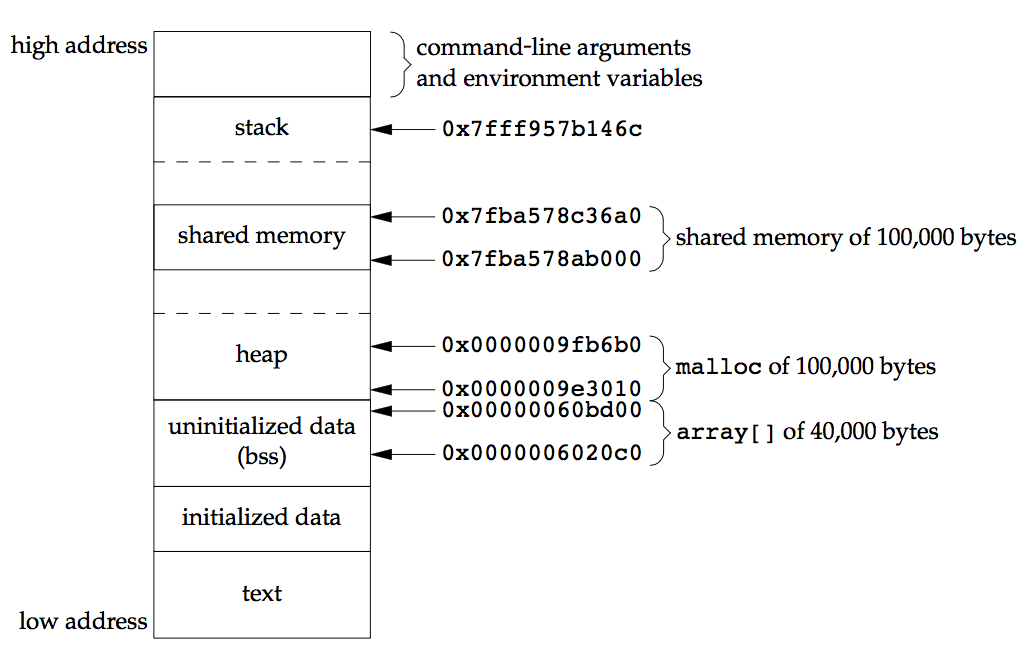
\includegraphics[width=0.9\textwidth]{figures/fig15_32-memory.png}
    \caption{Memory layout on an Intel-based Linux System}
  \end{figure}
\end{frame}



\begin{frame}[t,fragile, allowframebreaks]
  \frametitle{Shared Memory Example: Server - Client}
\texttt{codes/shm\_send.c}
\lstinputlisting[lineskip=-3pt]{codes/shm_send.c}

\newpage
\texttt{codes/shm\_receive.c}
\lstinputlisting[lineskip=-3pt]{codes/shm_receive.c}
\end{frame}


\begin{comment}
%---------------------------------------------------------

\section{Last Words}

\begin{frame}[t]
  \frametitle{Last Words}

\begin{itemize}
\item prepare for the exam
\end{itemize}
\end{frame}

\end{comment}

\end{document}
